%%%%%%%%%%%%%%%%%%%%%%%%%%%%%%%%%%%%%%%%%
% UNSW School of Physics
% LaTeX Assignment Template
% Version 1.0 (Updated 21/02/17)
% Last update by Adam Micolich
%%%%%%%%%%%%%%%%%%%%%%%%%%%%%%%%%%%%%%%%%

% Packages and other configurations for document

\documentclass[paper=a4, fontsize=12pt]{scrartcl}

\usepackage{url}
\usepackage{amsmath}

\usepackage{hyperref}
\usepackage{graphicx}
\newcommand{\cev}[1]{\reflectbox{\ensuremath{\vec{\reflectbox{\ensuremath{#1}}}}}}

\usepackage[T1]{fontenc} % Use 8-bit encoding that has 256 glyphs
\usepackage{fourier} % Use the Adobe Utopia font for the document - comment this line to return to the LaTeX default
\usepackage[english]{babel} % English language/hyphenation
\usepackage{amsmath,amsfonts,amsthm} % Math packages
\usepackage{graphicx} % Graphics packages
\usepackage{enumitem} % Lettered List Package
\usepackage{tikz} % Diagram Package
\usepackage{xcolor} % Colour Package
\usepackage{bm} % Bold Maths
\usepackage{caption} % Table titles

\usepackage{listings} % Code formatting
\usepackage{color}
 
\definecolor{codegreen}{rgb}{0,0.6,0}
\definecolor{codegray}{rgb}{0.5,0.5,0.5}
\definecolor{codeorange}{rgb}{0.7,0.2,0}
\definecolor{codered}{rgb}{0.7,0,0}
\definecolor{backcolour}{rgb}{0.95,0.95,0.92}
 
\lstdefinestyle{mystyle}{
    backgroundcolor=\color{backcolour},   
    commentstyle=\color{codered},
    keywordstyle=\color{codeorange},
    numberstyle=\tiny\color{codegray},
    stringstyle=\color{codegreen},
    basicstyle=\footnotesize,
    breakatwhitespace=false,         
    breaklines=true,                 
    captionpos=b,                    
    keepspaces=true,                 
    numbers=left,                    
    numbersep=5pt,                  
    showspaces=false,                
    showstringspaces=false,
    showtabs=false,                  
    tabsize=2
}
 
\lstset{style=mystyle}

% Block below sets up headers and sectioning.
\usepackage{fancyhdr} % Custom headers and footers
\pagestyle{fancy} % Makes all pages in the document conform to the custom headers and footers
\fancyhead[L]{z5173159 Cecilia Xifei Ni} %Page header left -- Student number and name
\fancyhead[C] {} %Page header center -- Empty
\fancyhead[R]{Word Embedding and Question Answering} %Page header right -- Course/year
\fancyfoot[L]{} % Empty left footer
\fancyfoot[C]{\thepage} % center footer -- page numbering
\fancyfoot[R]{} % Empty right footer
\renewcommand{\headrulewidth}{0pt} % Remove header underlines
\renewcommand{\footrulewidth}{0pt} % Remove footer underlines
\setlength{\headheight}{12pt} % Customize the height of the header
%\numberwithin{equation}{section} % Number equations within sections (i.e. 1.1, 1.2, 2.1, 2.2 instead of 1, 2, 3, 4)
%\numberwithin{figure}{section} % Number figures within sections (i.e. 1.1, 1.2, 2.1, 2.2 instead of 1, 2, 3, 4)
%\numberwithin{table}{section} % Number tables within sections (i.e. 1.1, 1.2, 2.1, 2.2 instead of 1, 2, 3, 4)
%\setlength\parindent{0pt} % Removes all indentation from paragraphs - comment this line for an assignment with lots of text

\usepackage{sectsty} % Allows customizing section commands
\allsectionsfont{\normalfont\scshape} % Make all sections default font with small caps
\renewcommand\thesection{} % Stops from putting section numbers in section headers but keeps numbering working.
\renewcommand\thesubsection{} % Stops from putting section numbers in section headers but keeps numbering working.
\renewcommand\thesubsubsection{} % See above

\usepackage{lipsum} % Inserts dummy latin text into template -- Can remove from final submission

% Title block on first page

\newcommand{\horrule}[1]{\rule{\linewidth}{#1}} % Create horizontal rule command with 1 argument of height

\title{	\normalfont \normalsize
\textsc{UNSW School of Computer Science and Engineering} \\ [24pt]
\horrule{1pt} \\[0.5cm] % Thin top horizontal rule
\LARGE Word Embedding and Question Answering \\ % The assignment title
\horrule{1pt} \\[0.5cm] % Thick bottom horizontal rule
}

\author{Cecilia Xifei Ni z5173159} % Your name

\date{\normalsize\today} % Today's date or a custom date

\begin{document}\thispagestyle{empty}

\maketitle % Print the title
\section{Introduction}
\begin{figure}
  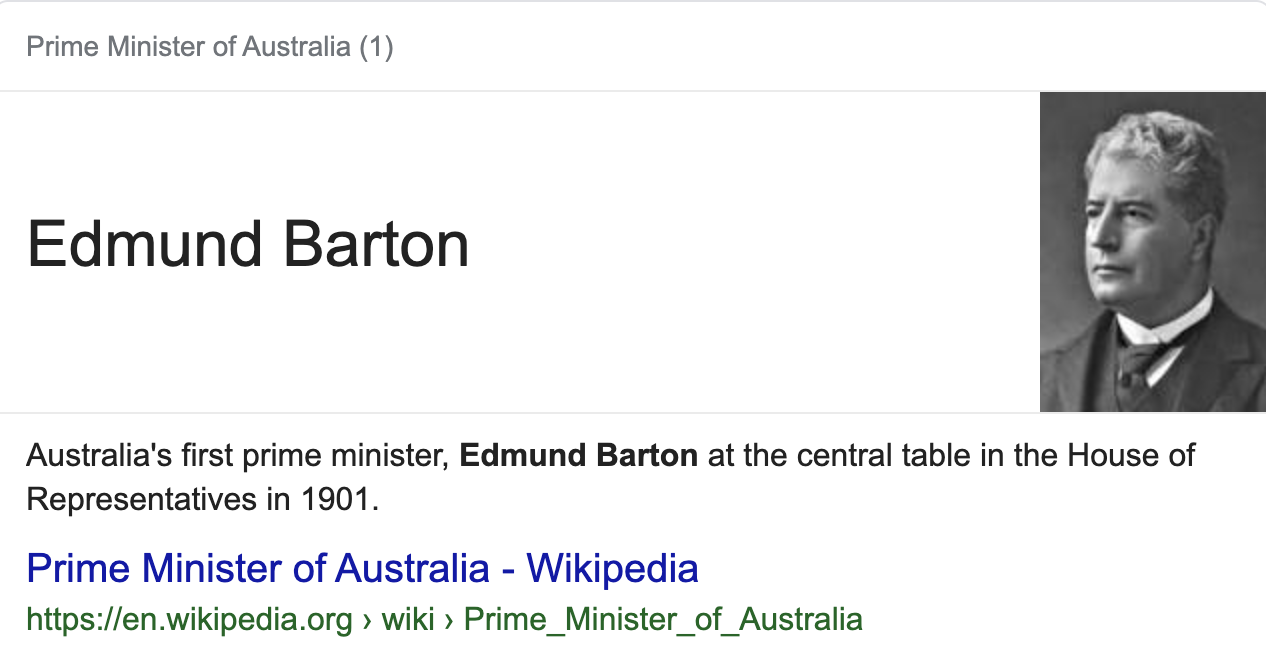
\includegraphics[width=\linewidth]{google.png}
  \caption{A result returned by Google to answer "Who is the first Prime Minister of Australia?"}
  \label{fig:google}
\end{figure}
"Who is the first Prime Minister of Australia?" \\\\
%% insert image
Figure 1 is a screen shot of search result returning by Google. This is a question a Question Answering (QA) system should be able to respond to. QA system evaluates texts across the web or database to find answer of a particular question to return in a form of short text.\\\\
Current machine algorithms extracts answer from a short paragraph instead of a long content (e.g. an entire wiki page/a news article). When applying modern machine learning algorithms on a long content, the result can be complicated and lenthy. \\\\
This essay aims to firstly gives a mathematical heavy explanation on nowadays natural language processing (NLP) algorithms on word embedding, then propose my own heuristics based on them to predict answers from a long content based on the question being asked. \\\\
My algorithm will be tested with \href{https://ai.google.com/research/NaturalQuestions/dataset}{Google Natural Questions} which contains its own private testing dataset. 
\section{General Word Embedding Models}
\textbf{Word Embedding} is the collective name for techniques in NLP  where words or phrases are mapped into vectors of real numbers. \\\\
As per all machine learning algorithms, the general philosophy is to find the minimum of a converged function. When trying to convert words to number, its original utf code will not work well. What we need is a hard-coded map between the word itself, and its semantics. As human, we learn these semantics from daily experience which machine has no way to access, therefore, we need a mapping from words and its semantic in order for machine to decode.
\subsection{First Attempt: Hot One Encoding}
Given a collection of $N$ unique words, each word is of size $N$. The vector is very sparse such that only one index is 1 and others are 0. This is to say each word is a \textbf{dimension}. \\\\
\begin{figure}
  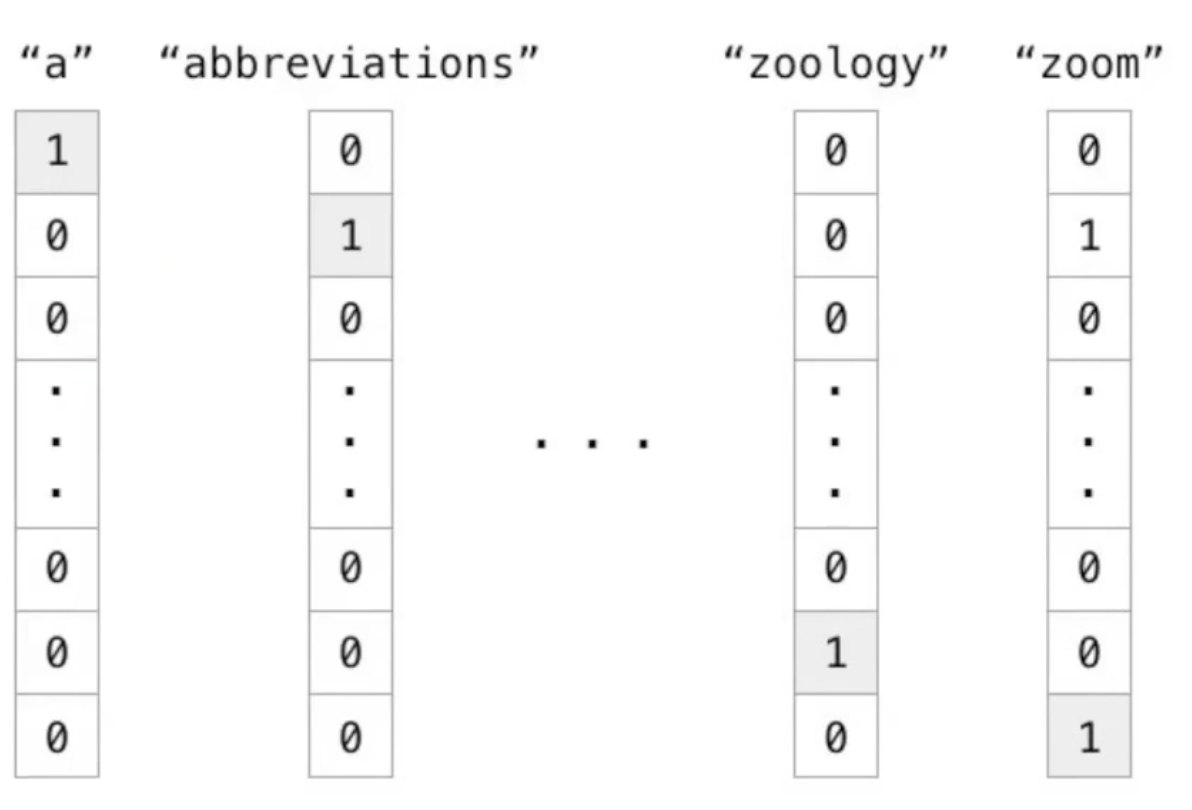
\includegraphics[width=\linewidth]{vectors.png}
  \caption{One Hot Encoding Example.}
  \label{fig:vector}
\end{figure}
Figure \ref{fig:vector} shows an example of hot encoding. \\\\
However, this model has some significant drawbacks. Firstly, it probably works fine for English as it has roughly 8000 frequent words. However, for languages like Chinese or Japanese, they are character-based, and each character will generate tons of combinations. This model will suffer from dramatic increase in dimensionalities. Secondly, all vectors in the matrix are independent to each other, while we do want them to learn the inter-connections between them.

\subsection{Second Attempt: Bag of Words (BoW) Model}
 On the second attempt, we focus more on extracting information from the perspective of the whole document. Under this model, we represent words in a document as a bag (multiset) of words-- we discard order and grammar, and only keep its multiplicity.\\\\
Here is an example:\\
Document 1: "George" "likes" "to" "play" "video" "games", "Mary" "likes" "video" "games" "too".\\
Document 2: "Mary" "also" "likes" "movies".\\\\
The BoW representation of the two above documentations is\\\\
BoW1: \{"George" : 1, "likes : 2", "to" : 1, "play " : 2, "video" : 2, "games" : 2, "Mary" : 1,  "too": 1\}\\
BoW2: \{"Mary" : 1, "also" : 1, "likes": 1, "movie" : 1\}\\
Here, each key is the word, and the value corresponds to occurrence. \\
\begin{figure}
  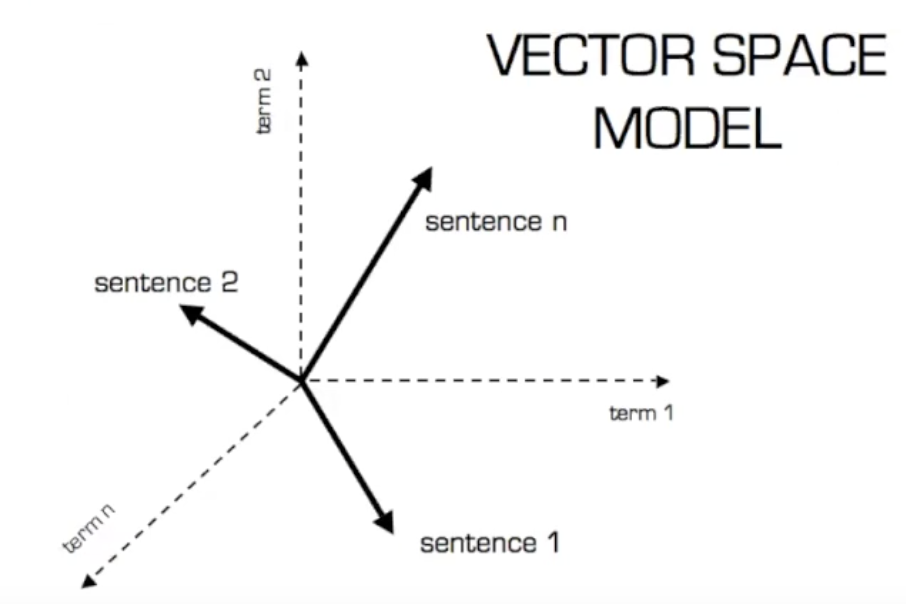
\includegraphics[width=\linewidth]{bow.png}
  \caption{Bag of Words Vector Space Representation}
  \label{fig:bow}
\end{figure}
This approach could be potentially used to compare similarities between two documents. When comparing them, we construct two vectors with each index corresponding to each unique words. Each be the count of the word appeared in that specific document. 
% more on cosine similarities/ euclidean distance.
The similarities of two documents can be measured by its Euclidean distance or its consine similarities. \\\\
Intuitively, two documents are similar if their vector points to the similar direction. We define the cosine similarities of two documents as: \\
\begin{align}
cosim(U_k, U_i) = \frac{\langle U_k, U_i \rangle}{\lVert U_k \rVert \cdot \lVert U_i \rVert}
\end{align}
where $\langle U_k, U_i \rangle$ is the scalar product of $U_i$ and $U_k$. 

\subsection{Third Attempt: Neural Network Based (NNLM)}
One intuitive question to ask is, Bag of Words and One Hot Encoding both treat each words as a separate dimension, but do we need so many dimensions?\\\\
The answer is probably no. Because a lot of words are similar or related. e.g. \\\\
Nouns: dog, cat, pet.\\
Verbs: fish, fished, fishing. \\
Adjective: very, great, significant. \\
Context: play {guitar, piano, games, tennis}\\\\
To not feel overwhelmed by the math at first, let's start with a easy example: \\
Words to be processed: boy, girl, woman, man \\
We can simply divide these words into two dimensions: gender and age as per Table 1 shows. This method is called \textbf{Distributed Representation}.\\\\
However, human language are so complex that we are not able to pre-define all dimensions for all words. Therefore we want to train a function $\mathbf{f}$ to get the word embedding for us. Figure 4 shows the function mapping. \\\\
To the best of my knowledge, we can do this in two ways. 
\begin{table}[]
\begin{tabular}{|l|l|l|}
\hline
       & 0     & 1      \\ \hline
gender & male  & female \\ \hline
age    & child & adult  \\ \hline
\end{tabular}
\caption{Table 1: Represent Words in Fewer Dimensions}
\end{table}

\begin{figure}
  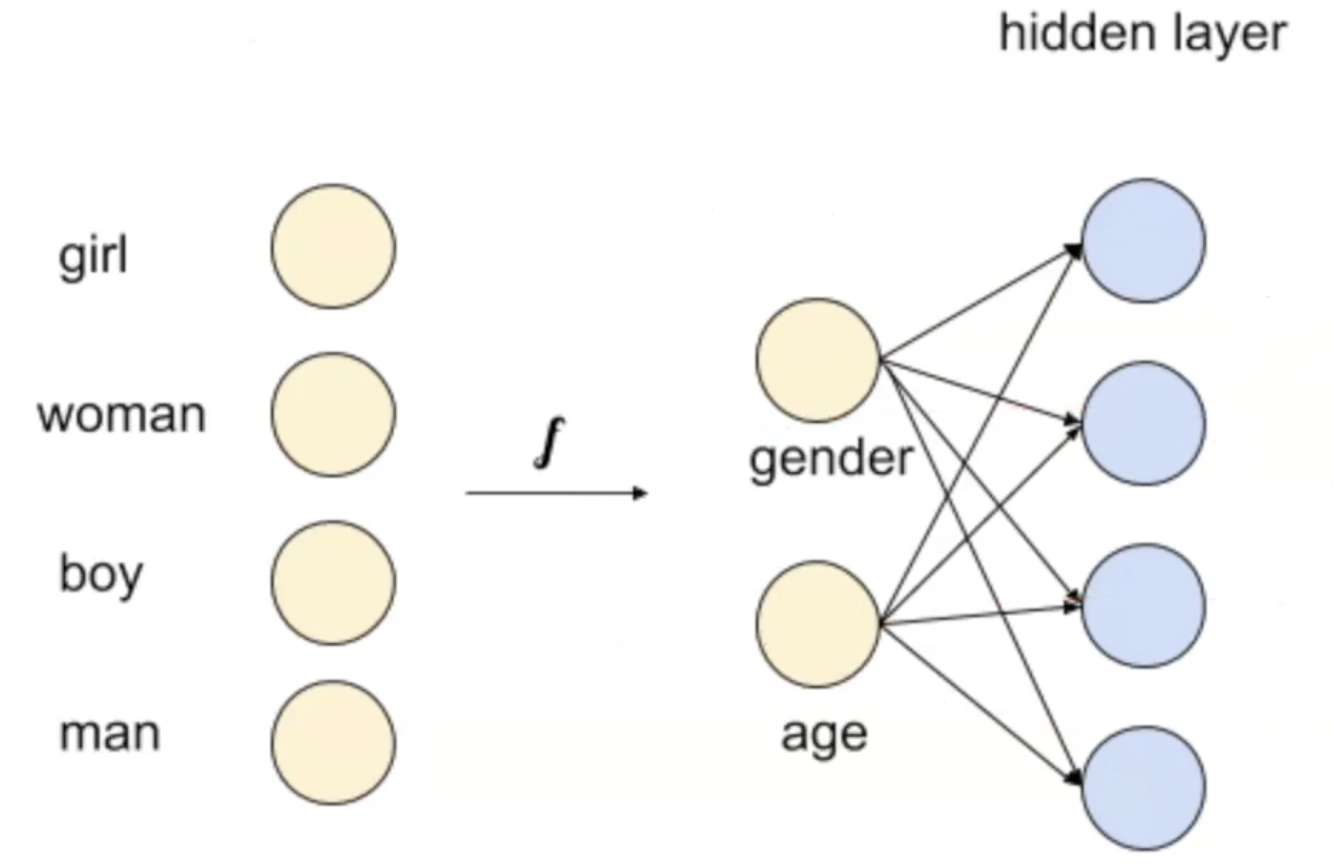
\includegraphics[width=\linewidth]{nnlm.png}
  \caption{Figure 4: Neural Network Based Mapping}
  \label{fig:nnlm}
\end{figure}
\subsubsection{Autoencoder (GAN)}
An autoencoder is a type of neural network that learns to label dimensions in an unsupervised manner. Figure 5 shows that an autoencoder is composed of two parts: the input side, marked as $X$, and the reconstruction (output) side, marked as $X'$. The $X$ tries to learn a distributed representation of the original data that aims to reduce the dimensions, and the $X'$ side is where the autoencoder tries to generate from the reduced representation as close as possible to its original input, hence its name, reconstruction. 
\begin{figure}
  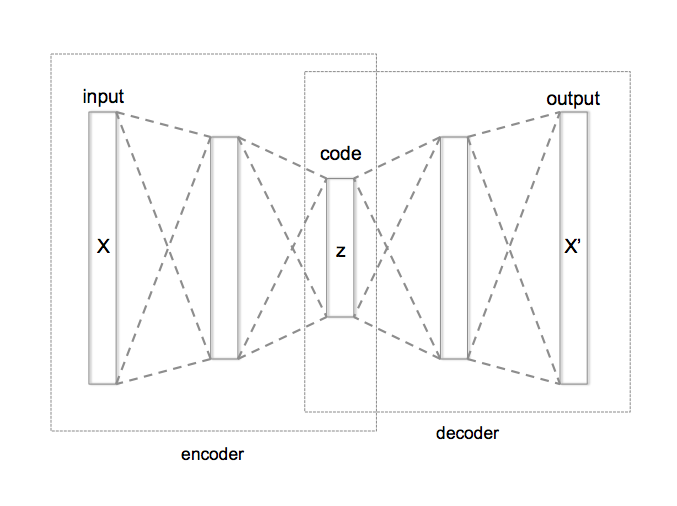
\includegraphics[width=\linewidth]{Autoencoder_structure.png}
  \caption{Schematic structure of an autoencoder with 3 fully connected hidden layers. The code (z, or h for reference in the text) is the most internal layer.}
  \label{fig:autoencoder}
\end{figure}
\paragraph{Basic Architecture of Autoencoder}
An autoencoder consists of two parts, the encoder and the decoder, which can be defined as transitions $\psi$ and $\phi$, such that:
\begin{align*}
& \psi : \chi \mapsto \mathfrak{F} \\
& \phi : \mathfrak{F} \mapsto \chi \\
& \psi, \phi = arg_{\psi, \phi} min \lvert \chi - (\psi * \phi) \chi \rvert
\end{align*}
In the simplest form, we assume there is only one hidden layer. The encoder stage of the autoencoder takes input $x \in \mathbb{R}^{d} = \chi$ and maps it to $\mathbf{h} \in \mathbb{R}^{p} = \mathfrak{F}$. \\
\begin{align*}
\mathbf{h} = \delta (\mathbf{W}x + \mathbf{b})
\end{align*}
This image $\mathbf{h}$ is the code section shown in Figure 5. $\delta$ is normally a sigmoid function defined as following: \\
\begin{align*}
S(x) = \frac{1}{1 + e^{-x}} = \frac{e^x}{e^x + 1}
\end{align*}
$\mathbf{W}$ is a weight matrix and $\mathbf{b}$ is a bias vector. The initializations of these two variables are random. They will be learnt iteratively through \textbf{backpropagation}. \\
\begin{align*}
\mathbf{h'} = \sigma (\mathbf{W'}x + \mathbf{b'})
\end{align*}
The backpropagation computes weight space $\mathbf{W}$ and bias vector $b$ with respect of a loss function $\mathbb{C}$.\\\\
$x$ : input (vector of features). \\
$x'$ : target output, the closer to $x$, the better. \\
$\mathbb{C}$: loss function, which intuitively associate with the "cost" of certain event or representation. The aim of training is to minimize the loss function. \\
$L$: the number of layers. In the above example, L equals to 1. However, here we aims to provide a generalized form.\\
$W^l = W^l_{j_k}$: the weights between layer  $l-1$ and $l$, where $W^l_{j_k}$ is the weight between the k-th node in layer $l$-1 and the $j$-th node in layer $l$.\\
$f^l$: sigmoid function at layer $l$.\\
The whole neural network can be represented by this function:\\
\begin{align*}
g(x) = f^{L}(W^Lf^{L-1}(W^{L-1}...f^1(W^1*x)...)
\end{align*}
For each input $x_i$, there will be an output $x'_i$ corresponding with it. the loss of the model on that pair is the cost of the difference between the predicted output $g(x_i)$  and the target output $x'_i$:\\
\begin{align*}
\mathbb{C}(y_i, f^{L}(W^Lf^{L-1}(W^{L-1}...f^1(W^1*x)...))
\end{align*}
For each layer, we compute the minimum of the loss function by calculating its derivatives. 
\begin{align*}
\frac{\partial \mathbb{C}}{\partial W^l_{j_k}}
\end{align*}
Where the loss function is defined as: 
\begin{align*}
\mathbb{C}(x, x') = \lvert x - x'\rvert^2 = \lvert x - \sigma'(\mathbf{W}'(\sigma (\mathbf{W}x + b)) + b' \rvert
\end{align*}
where $x$ is the average across all inputs.
\subsubsection{Neural Network Language Model (NNLM)}
However, the above model does not fully utilize the context of words, as in words in this category:\\
Context: play {guitar, piano, games, tennis}\\\\
More specifically, autoencoder does generate vectors that significantly reduce the dimensions compared to previous attempts but it takes into account less than 1 or two words, hence it is not so great at predicting the next word based on the previous context. \\
Bengio proposed the following model that makes use of the word order in a document. It can be presented by the conditional probability of the next word given all the previous ones:
\begin{align*}
\hat{P} (w^{T}_1) = \prod^T_{t=1} \hat{P} (w_t | w^{t-1}_1)
\end{align*}
where $w_t$ is the t-th word.\\\\
In more details: \\\\
The training set is $w_1, w_2, ... w_t \in V$, where $V$ is the vocabulary set that is roughly of size $10^5$ depending on language. \\
We need to learn $f(w_t, ..., w_{t-n+1})= \hat{P} (w_t | w^{t-1}_1)$, in the sense it gives highest likelihood of the next word.\\
This is subject to constraints that: \\
For any choice of $w^{t-1}_1$
\begin{align*}
& \sum_{i=1}^{\lvert V \rvert} f(i, w_t, ..., w_{t-n+1}) = 1 \\
& f > 0
\end{align*}
The function $f(w_t, ..., w_{t-n+1})= \hat{P} (w_t | w^{t-1}_1)$ has two parts: \\
 1. $\mathbb{C}$ : $w_i \rightarrow \mathbb{C}(w_i) \in \mathbb{R}^m$ where $m$ ranges from 30 to 100, which is significant smaller than the size of $V$ and $w_i \in V$.\\
 2. A probability function over words: \\
 A function $g$ that maps an input sequence of words $(\mathbb{C}(w_{t-n+1}), ..., \mathbb{C}(w_{t-1})$ to the next word $w_t \in V$.
 \begin{align*}
 f(i, w_t, ..., w_{t-n+1}) = g(i, \mathbb{C}(w_{t-1}, ...,  C(w_{t-n+1}))
 \end{align*}
 $\mathbb{C}$ is being shared for the whole neural network. $\mathbb{C}$ simply maps a word $w_t \in V$ to a \textit{feature vector} of $\mathbb{R}^m$ shown as \textbf{figure 7}.\\\\
 \begin{figure}
  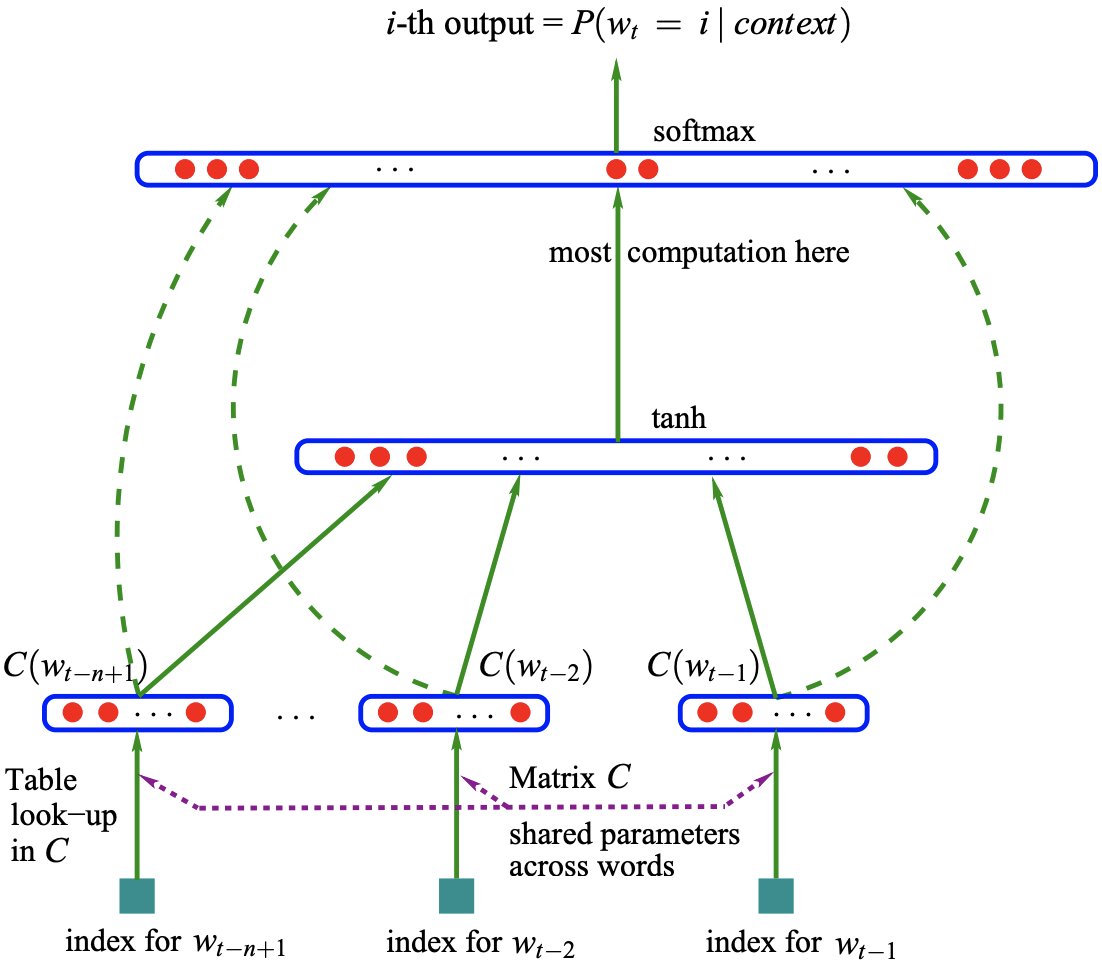
\includegraphics[width=\linewidth]{neuralnet.png}
  \caption{Neural Architecture}
  \label{fig:nnlm}
\end{figure}
The function $g$ might be implemented by a feed-forward or recurrent neural network with parameter $\omega$. The overall parameter set is $\theta = (\mathbb{C}, \omega)$\\\\
Training aims to maximize $\omega$ the log-likelihood.
\begin{align*}
L = \frac{1}{T}\sum_{t}log f(w_t, w_{t-1}, ..., w_{t-n+1}; \theta) + R(\theta)
\end{align*}
where $R$ is a regularization form. \\\\
The \textit{softmax} output layer in figure 7 grants the positive probabilities summing up to 1:
\begin{align*}
\hat{P}(w_t | w_{t-1}, ..., w_{t-n+1}) = \frac{e^{yw_t}}{\sum_{i} e^{y_i}}
\end{align*}
The $y_i$ is the log probability for each possible output word $w_i \in V$, defined as follows:
\begin{align*}
y = b+Wx+U tanh(d +Hx)
\end{align*}
as figure 7 shows, $tanh$ is applied on each word. $W$ is the weight matrix we described in the previous attempt. $x$ is the word feature activation vector that is a concatenation from $\mathbb{C}(w_i)$
\begin{align*}
x = \mathbb{C}(w_{t-1}), \mathbb{C}(w_{t-1}), ..., \mathbb{C}(w_{t-n+1})
\end{align*}
$b$ and $d$ are biases which are addictive parameter in neural networks that only have outgoing edges but no incoming edges. Its existence is mainly to not let function passing the origin. 
Here is a intuitive example of training results: \\
\texttt{cat} and \texttt{dog} plays similar role in linguistic, syntactically and semantically. \texttt{backyard} and \texttt{frontyard} also plays similar role. \texttt{running} and \texttt{walking} is also a pair. \texttt{is} and \texttt{was} are also quite similar. \\
From the probability mass of them, we can simply transform:\\
\texttt{A cat is walking at frontyard} \\
to \texttt{A dog is walking at the frontyard} \\
to \texttt{A dog is running at the frontyard} \\
to \texttt{A dog was running at the frontyard} \\
to \texttt{A dog was running at the backyard}
\subsection{Fourth Attempt: Word2Vec}
The above attempt only considers "context" before certain word. However, in 2013, a paper published by Mikolov and Jeff Dean proposed a famous model, Word2Vec, that considers bidirectional context, i.e. context before and after the predicting word. \\\\
It has a very similar structure as the attempt we elaborated above, but it is more focusing on \textbf{Word Embedding}, i.e. representing a word in vector form,  instead of predicting the word based on preceding context.\\\\
Word2Vec is a two-layer neural net that takes a input word and output it as a feature vector. The core purpose is to gather similar word into the same vector space by calculatingthe probabilities --the likelihood that they will co-occur.\\\\
It has the following two approaches. 
\subsubsection{Continuous Bag-of-Word (CBOW)}
 \begin{figure}
  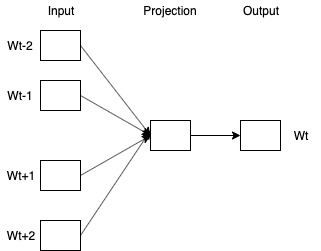
\includegraphics[scale=1]{cbow.jpg}
  \caption{Continuous Bag-of-Words}
  \label{fig:cbow}
\end{figure}
The aim of CBOW is the predict the middle word given the words surrounding it. \\
For example, \textit{ \{ I ?? video games \}} $\rightarrow$ \textit{\{play\}}\\\\
As figure 7 shows, this is quite similar to the feed-forward neural network described above.  It removes all the hidden layers, and its projection layer is shared among all words, where the projection layer is either sum or average of all the vectors of the words. Note that despite its name being "Bag-of-words", it bears no relevance to the first attempt we mentioned above. 
\subsubsection{Continuous Skip-gram(Skip Gram)}
 \begin{figure}
  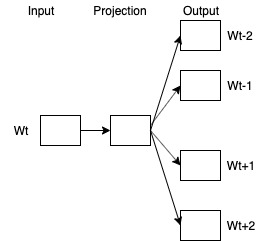
\includegraphics[scale=1]{skip-gram.jpg}
  \caption{Continuous Skip-Gram}
  \label{fig:skip-gram}
\end{figure}
Opposite to CBOW model, the objective of \textit{skip gram} is to predict surrounding words from a single word, as shown in figure 8.\\\\
Given a sequence of words $w_1, w_2, w_3, ..., w_n$, similar to the maximization of log-likelihood described in the third attempt, the goal of the Skip-gram model is to maximize the average log probability:
\begin{align*}
\frac{1}{T}\sum_{t=1}^{T} \sum_{-c \leq j \leq c, j \neq 0} log p (w_{t+j} | w_t)
\end{align*}
where $c$ is the training size. Obviously, larger $c$ will lead to higher accuracy, in the cost of trading run time. We define $p (w_{t+j} | w_t)$ using the \textit{softmax} function. 
\begin{align*}
p(w_O | w_I) = \frac{exp(x^T_{w_O}  v_{w_I})}{\sum^W_{w=1}exp(x^T_{w_O} v_{w_I})}
\end{align*}
where $x_w$ and $v_w$ are input and output shown in \textbf{figure 8}. $W$ is the size of vocabulary in the language we trained in. 
\subsubsection{Refinement of Word2Vec}
\textbf{Word2Vec} is a quite expensive algorithm just because of the significant time it takes to run it. \\
The training complexity of the architecture is proportional to  
\begin{align*}
Q = C \times (D + D \times log_2(V ))
\end{align*}
where $C$ is the maximum distance of the words.\\\\
However. there are several ways we can improve its run-time.
\subparagraph{Hierarchical Softmax}
This model in natural probabilistic language was firstly proposed by Morin and Bengio. The main advantage is that this model improves searching $W$ to $log_2{W}$.\\\\
 \begin{figure}
  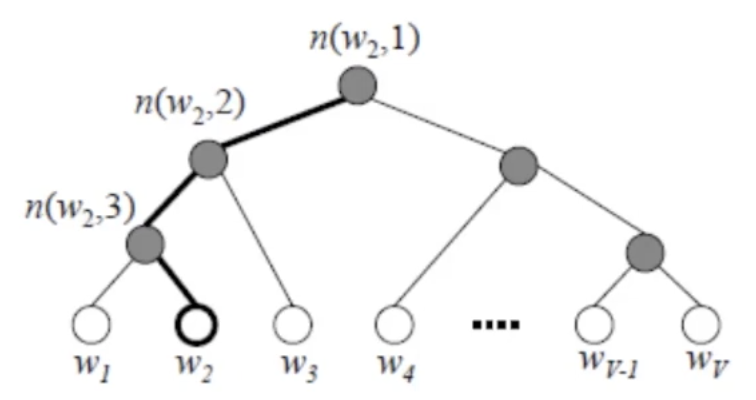
\includegraphics[scale=1]{softmax.png}
  \caption{Hierarchical Softmax Model}
  \label{fig:skip-gram}
\end{figure}
The \textbf{Hierarchical Softmax} uses a binary tree representation that represents $W$ words. For each node, its child nodes' probabilities are explicitly represented. \\\\
More intuitively, each node can be reached by traversing from the root of the tree. Nodes that are further down the tree have less probability of being selected as output. \\\\
Let $n(w, j)$ be the $j$-th node on the path from root $w$, and let $L(w)$ be the length of the path. therefore,
\begin{align*}
& n(w, 1) = root \\
& n(w, L(w)) = w
\end{align*}
For any inner node $n$, let $mid(n)$ be an arbitrary fixed child of $n$, and define $\| x \|$ as
\[ \begin{cases} 
      0 & x \ is \  false\\
      1 & x \ is \ true
   \end{cases}
\]
Then we define \textbf{Hierarchical Softmax} $p(w_O | w_I)$ as follows
\begin{align*}
p(w_O | w_I) = \prod^{L(w)-1}_{j = 1} \sigma ( \| n(w, j + 1) = mid(n(w, j))\| x_{n(w, j)}^{T} v_{w_j} )
\end{align*}
where $\sigma$ is defined as
\begin{align*}
\sigma(x) = \frac{1}{1 + exp(-x)}
\end{align*}
Also
\begin{align*}
\sum^W_{w = 1} p(w | w_I) = 1
\end{align*}
The above fomulas indicates that the computational cost is proportional to $L(w_O)$, which on average is smaller than $logW$.
\subparagraph{Negative Sampling} This model has another name called \textbf{Noise Contrastive Estimation (NCE)}, and it was introduced by Gutmann and Hyvarinen.\\\\
NCE is roughly a maximum of log probability of the softmax that defines as follows:
\begin{align*}
log \sigma (x_{w_O}^{T} v_{w_I}) + \sum^{k}_{i = 1} \mathbb{E}_{w_i}~P_n(w) [log \sigma (-x_{w_O}^{T} v_{w_I}) ]
\end{align*}
$P_n(w)$ is a noise distribution serving as a free parameter in the above formula. 
Mikolov has observed a number
of choices for Pn(w) and found that the unigram distribution U(w) raised to the 3/4rd power(i.e.,$U(w)^{3/4}/Z$) outperformed significantly the unigram and the uniform distributions.
\subsubsection{Results of Word2Vec}
 \begin{figure}
  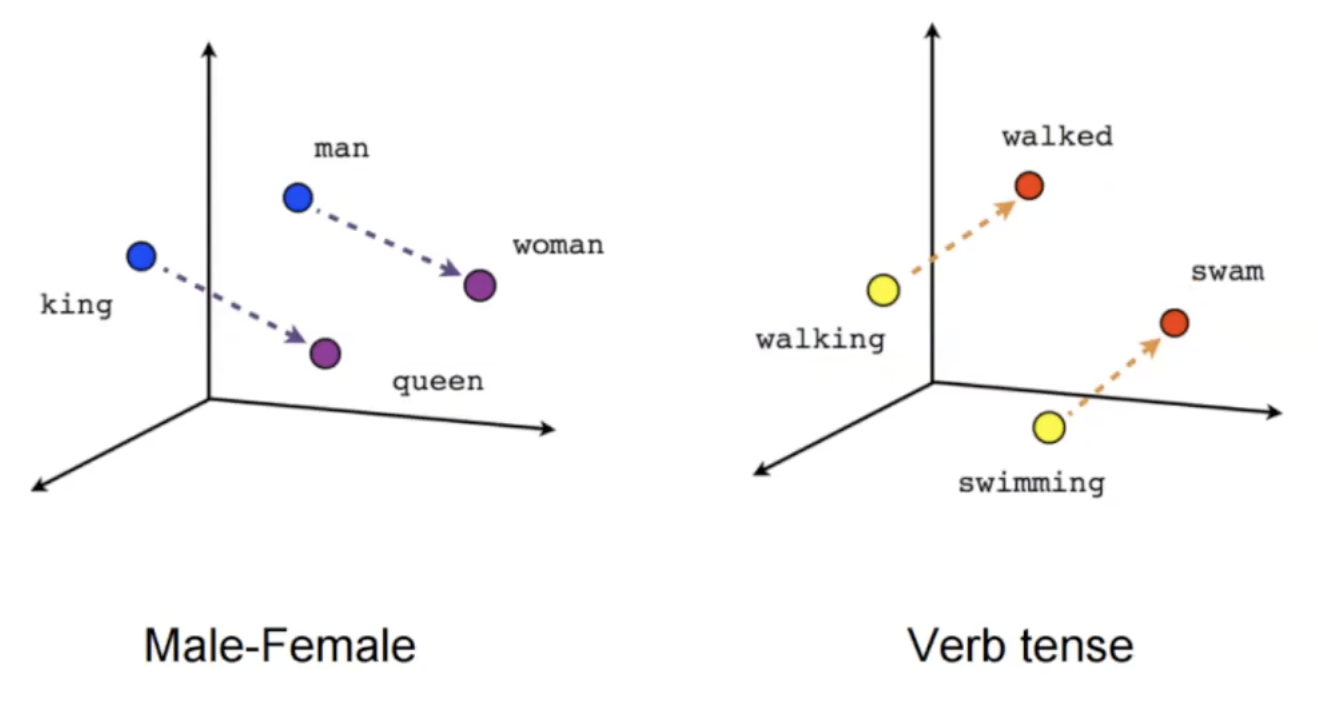
\includegraphics[scale=0.7]{word2vectorresult.png}
  \caption{Vector Space of Word2Vec}
  \label{fig:skip-gram}
\end{figure}
Figure 10 shows that \textbf{Word2Vec} can be successful in creating the vector representation of a word, for example, \texttt{king} and \texttt{queen} has a closer Euclidean distance, and a smaller angle in-between.\\\\
Moreover, with vector representation of a word, we can write formula based off words. For instance: \\
\texttt{France + Paris - Being = China} \\
The result of \texttt{France + Paris - Being} would be equal or very close to the value of   \texttt{Beijing}. \\\\
Isn't that interesting?
\subsection{Global Vectors for Word Representation (GloVe)}
This model is highly similar to \textbf{Word2Vec} introduced above. The only difference is \textbf{Word2Vec} looks for limited set of context surrounding the certain word, while \textbf{GloVe} calculates based on the whole document. Its training is performed on aggregated global word-word co-occurrence statistics from the corpus. Therefore, \textbf{GloVe} can only be offline, which is its main drawback. \\\\
This algorithm isn't used that frequently as the relevance between a word and its whole document is quite limited. 

\subsection{Embedding from Language Model (ELMo)}
 \begin{figure}
  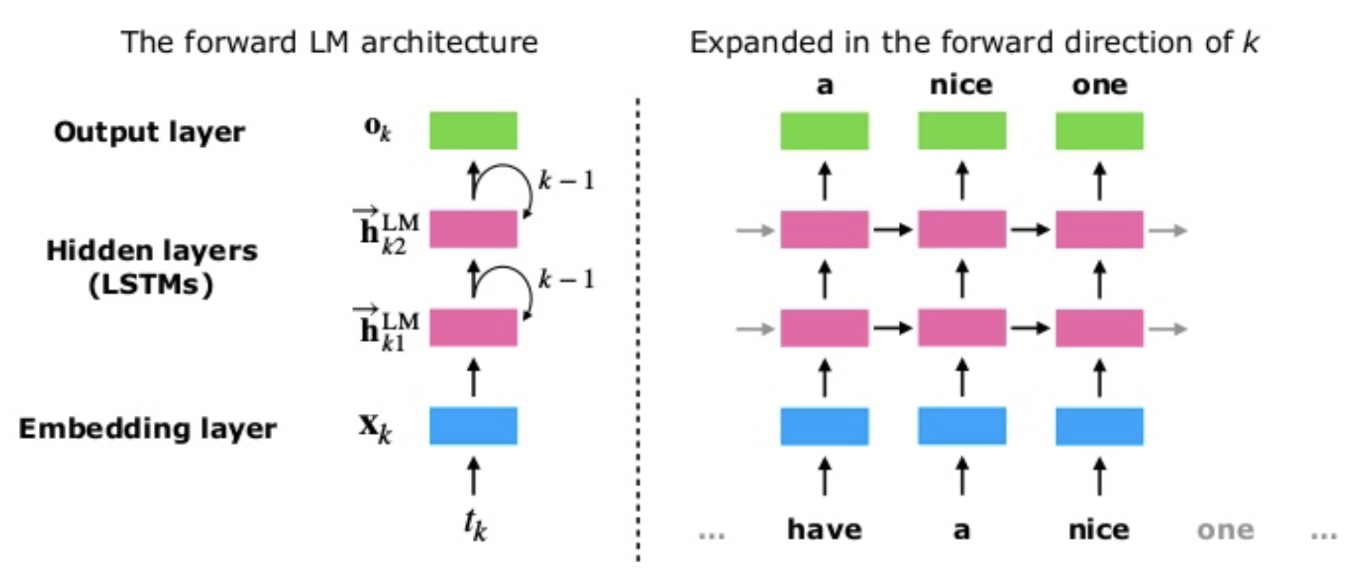
\includegraphics[scale=0.7]{ELMo.png}
  \caption{Two-layer Bidirectional LSTM Backbone}
  \label{fig:skip-gram}
\end{figure}
All the above models does not consider words with multiple meanings. Peters published a paper in 2018 of deep contextualized word representation that models complex characteristics of word use and how these uses vary across linguistic context. \\\\
Remarkably, previous models, after training, get constant vectors, while \textbf{ELMo} only gets a pre-trained vector. And the final output will be calculated after fine-tuning. So \textbf{ELMo} changes NLP from static to dynamic! \\\\
Given a sequence of $N$ tokens, $(t_1, t_2, t_3, ... t_N)$, we propose a forward language model that computes the probabilities of the sequence $t_k$ given all the history token $(t_1, t_2, t_3, ... t_k)$. 
\begin{align*}
p(t_1, t_2, t_3, ... t_N) = \prod^N_{k = 1} p(t_k | t_1, t_2, ... ,t_{k-1})
\end{align*}
The forward: \textbf{ELMo} uses LSTM layer to compute output. At the forward direction, for each position $k$, each LSTM layer outputs a context dependent representation $\vec{\mathbf{h}}^{L,M}_{k, j}$ where $j = 1, 2, 3, ..., L$. The top layer LSTM output $\vec{\mathbf{h}}^{L,M}_{k, j}$ is used to predict the next token $t_{k+1}$ with softmax. \\\\
The backward:  A backward LM is similar to a forward LM, except it runs over the sequence in reverse, predicting the previous token given the future context:
\begin{align*}
p(t_1, t_2, t_3, ... t_N) = \prod^N_{k = 1} p(t_k | t_{k+1}, t_{k+2}, ... ,t_N)
\end{align*}
Its implementation is also quite similar: we produce $\cev{\mathbf{h}}^{L, M}_{k, j}$ of $t_k$ given $(t_{k+1}, t_{k+2}, ... ,t_N)$\\\\
The formulation of \textbf{ELMo} jointly combines the forward and backward directions that maximize the log likelihood: 
\begin{align*}
\sum^N_{k=1} (logp (t_k | t_1, t_2, ..., t_{k-1}; \theta_x, \vec{\theta}_{LSTM}, \theta_{S}) + 
(logp (t_k | (t_{k+1}, t_{k+2}, ... ,t_N; \theta_x, \cev{\theta}_{LSTM}, \theta_{S})
\end{align*}
Hence, for each token $t_k$, \textbf{ELMo} computes a set of $2L+1$ representations. 
\begin{align*}
& R_k = \{x^{LM}_k, \vec{\mathbf{h}}^{L,M}_{k, j}, \cev{\mathbf{h}}^{L, M}_{k, j} | j = 1, ... L\} \\
& = \{ \mathbf{h}^{L, M}_{k, j} | j = 1, ... L\}
\end{align*}
where $\mathbf{h}^{L, M}_{k, j} $ is the token layer. \\\\
More generally, we compute a task specific weighting of all biLM layers:
\begin{align*}
ELMo^{task}_k = E(R_k ; \theta^{task} = \gamma^{task} \sum^{L}_{j=0} s^{task}_j \mathbf{h}^{L, M}_{k, j} 
\end{align*}
where $s^{task}$ is a softmax-nomalized weights and the $\gamma$ allows task to scale the entire \textbf{ELMo} vector. The indices k and j correspond to the index of the word and the index of the layer from which the hidden state is being extracted from.\\\\
 \begin{figure}
  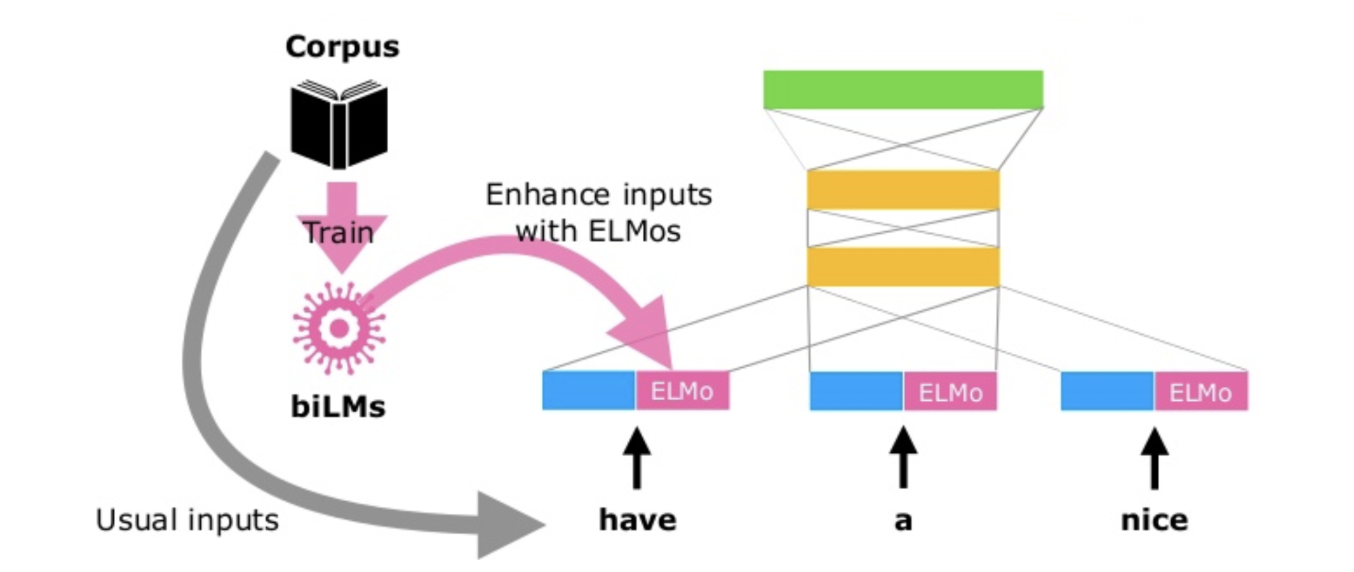
\includegraphics[scale=0.7]{elmoprocee.png}
  \caption{Overview of the procedure on training ELMo}
  \label{fig:skip-gram}
\end{figure}
To summarize:
$\bullet$ \textbf{ELMo} dynamically determines word embedding in downstream task \\\\
$\bullet$ ELMo generates three embeddings: \\
1. word embedding \\
2. 1st LSTM layer embedding \\
3. 2nd LSTM layer embedding \\
$\bullet$ the pre-training step involves getting three embedding $(v_1, v_2, v_3)$ per word. \\\\
$\bullet$ the fine-tuning step involves freezing the embedding and train weight $(w_1, w_2, w_3)$ for $(v_1, v_2, v_3)$ per word. \\\\
$\bullet$ The final embedding is $w_1 v_1 + w_2 v_2 + w_3 v_3$\\\\
Why three embeddings only? because normal words have less or equal to three meanings, and this is practically proven to work the best. 
 \begin{figure}
  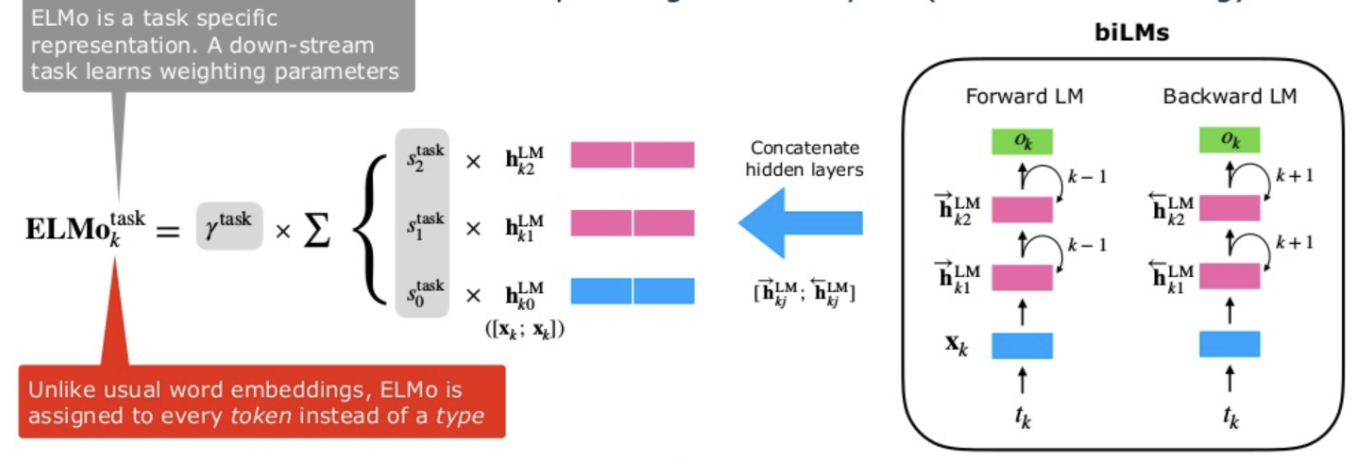
\includegraphics[scale=0.7]{elmofunction.png}
  \caption{A graphic elaboration on ELMo function}
  \label{fig:skip-gram}
\end{figure}
\subsection{Bidirectional Encoder Representation from Transformer (BERT)}
\textbf{BERT} is a model published by Google in 2018 Nov that basically takes advantage of all the previous models that we introduced. \\\\
Similar to \textbf{ELMo}, it has two phases: pre-training and fine-tuning, and it also utilizes two-layer bidirectional model. \\\\
Similar to \textbf{Word2Vec}, it also predicts word from a given context, and transform it to a vector.\\\\
It uses Transformer which is a model proposed in the famous paper \textit{Attention is All You Need} instead of RNN-GPT (Generative Pre-training).\\\\
In this report, we denote the number of layers, aka, Transformer Blocks, as $L$.\\
The hidden size as $H$. \\
The number of self-attention heads as $A$. 
\subsubsection{Transformer}
\subsubsection{Input/Output Representation}
The input of \textbf{BERT} can be both a sentence or a set of sentences, which is an arbitrary continuous text. \\\\
Then \textbf{BERT} uses WordPiece embeddings with a 30,000-token library. The first token of a sequence is normally a special classification token (\texttt{[CLS]}). The final hidden state of this token is used as the "aggregate sequence representation for classification tasks". Sentence pairs are packed together into a single sequence. \textbf{BERT} differentiate the sentences in two ways. \\\\
 First, \textbf{BERT} separate them with a special token (\texttt{[SEP]}). Second, \textbf{BERT} adds a learned embedding to every token implying the sentence it belongs, be it sentence \texttt{A} or sentence \texttt{B}. \\\\
As shown in \textbf{Figure 14}, \textbf{BERT} denotes the input embedding as \texttt{E}, the final hidden vector of the special \texttt{[CLS]} for the $i$-th input token as $T_i \in \mathbb{R}^H$
\subsubsection{Masked Language Model}
 \begin{figure}
  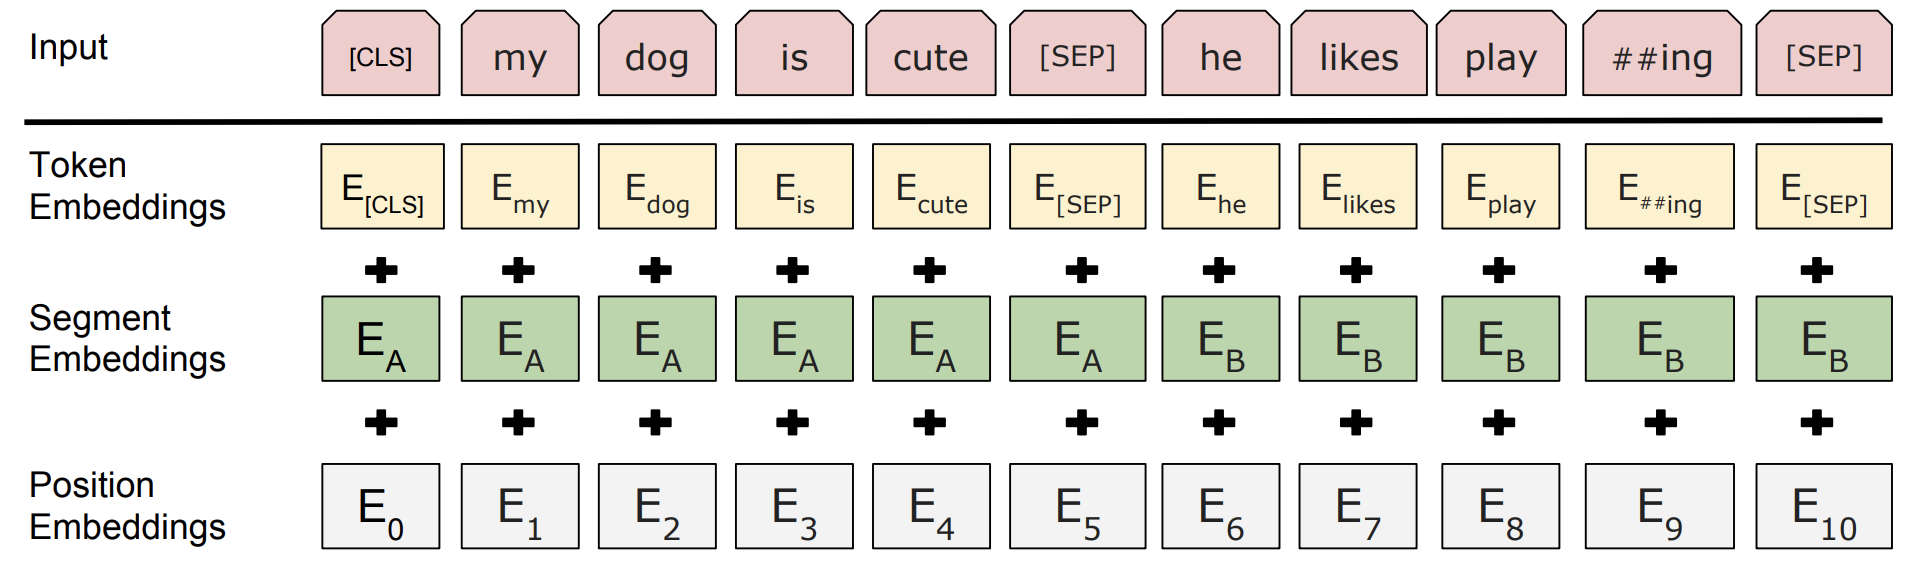
\includegraphics[scale=0.53]{bertinput.png}
  \caption{BERT input representation. The input embeddings are the sum of the token embeddings, the segmentation embeddings and the position embeddings.}
  \label{fig:skip-gram}
\end{figure}
Intuitively,  it is quite obvious that a bi-directional NLP model is better than models that purely considers left-to-right or right-to-left. Sadly, the conditional probability determines that the direction is either left-to-right or right-to-left. A bidirectional model requires the words to be predicted to see itself. \\\\
How \textbf{BERT} solves this problem is using a \textbf{Masked Language Model} (Masked LM in short). They mask random random tokens in the sequence, and the try to predict that. Unlike autoencoder that we elaborated above, \textbf{BERT} only predicts the masked words rather than reconstructing the entire input. \\\\
To address the difference between the pre-training and the fine-tuning stages, because of the mismatches created by words being replaced by \texttt{[MASK]}\\\\
Empirically, \textbf{BERT} randomly selects 15 \% of tokens as \texttt{[MASK]}, then only actually replace them with \texttt{[MASK]} in 80\%. Then, $T_i$ will be used to predict the original token with cross entropy loss.
\subsubsection{Next Sentence Predication (LSP)} 
A lot of important tasks in NLP such as \textbf{Question Answering} (QA), and \textbf{Natural Language Inference (NLI)} are grounded on the understanding of the \textit{relationship} between sentences. \\\\
Supposing that we have a sentence \texttt{A}, and a sentence \texttt{B} in the pre-training set, there's 50\% of the time where \texttt{B} is actually the sentence following \texttt{A}, in which case we mark \texttt{B} as \texttt{IsNext}, and for the rest of the times, \texttt{B} is just some random sentences from the document that bears no relationship with \texttt{A}-- in this case, we mark \texttt{B} as \texttt{NotNext}.
 \begin{figure}
  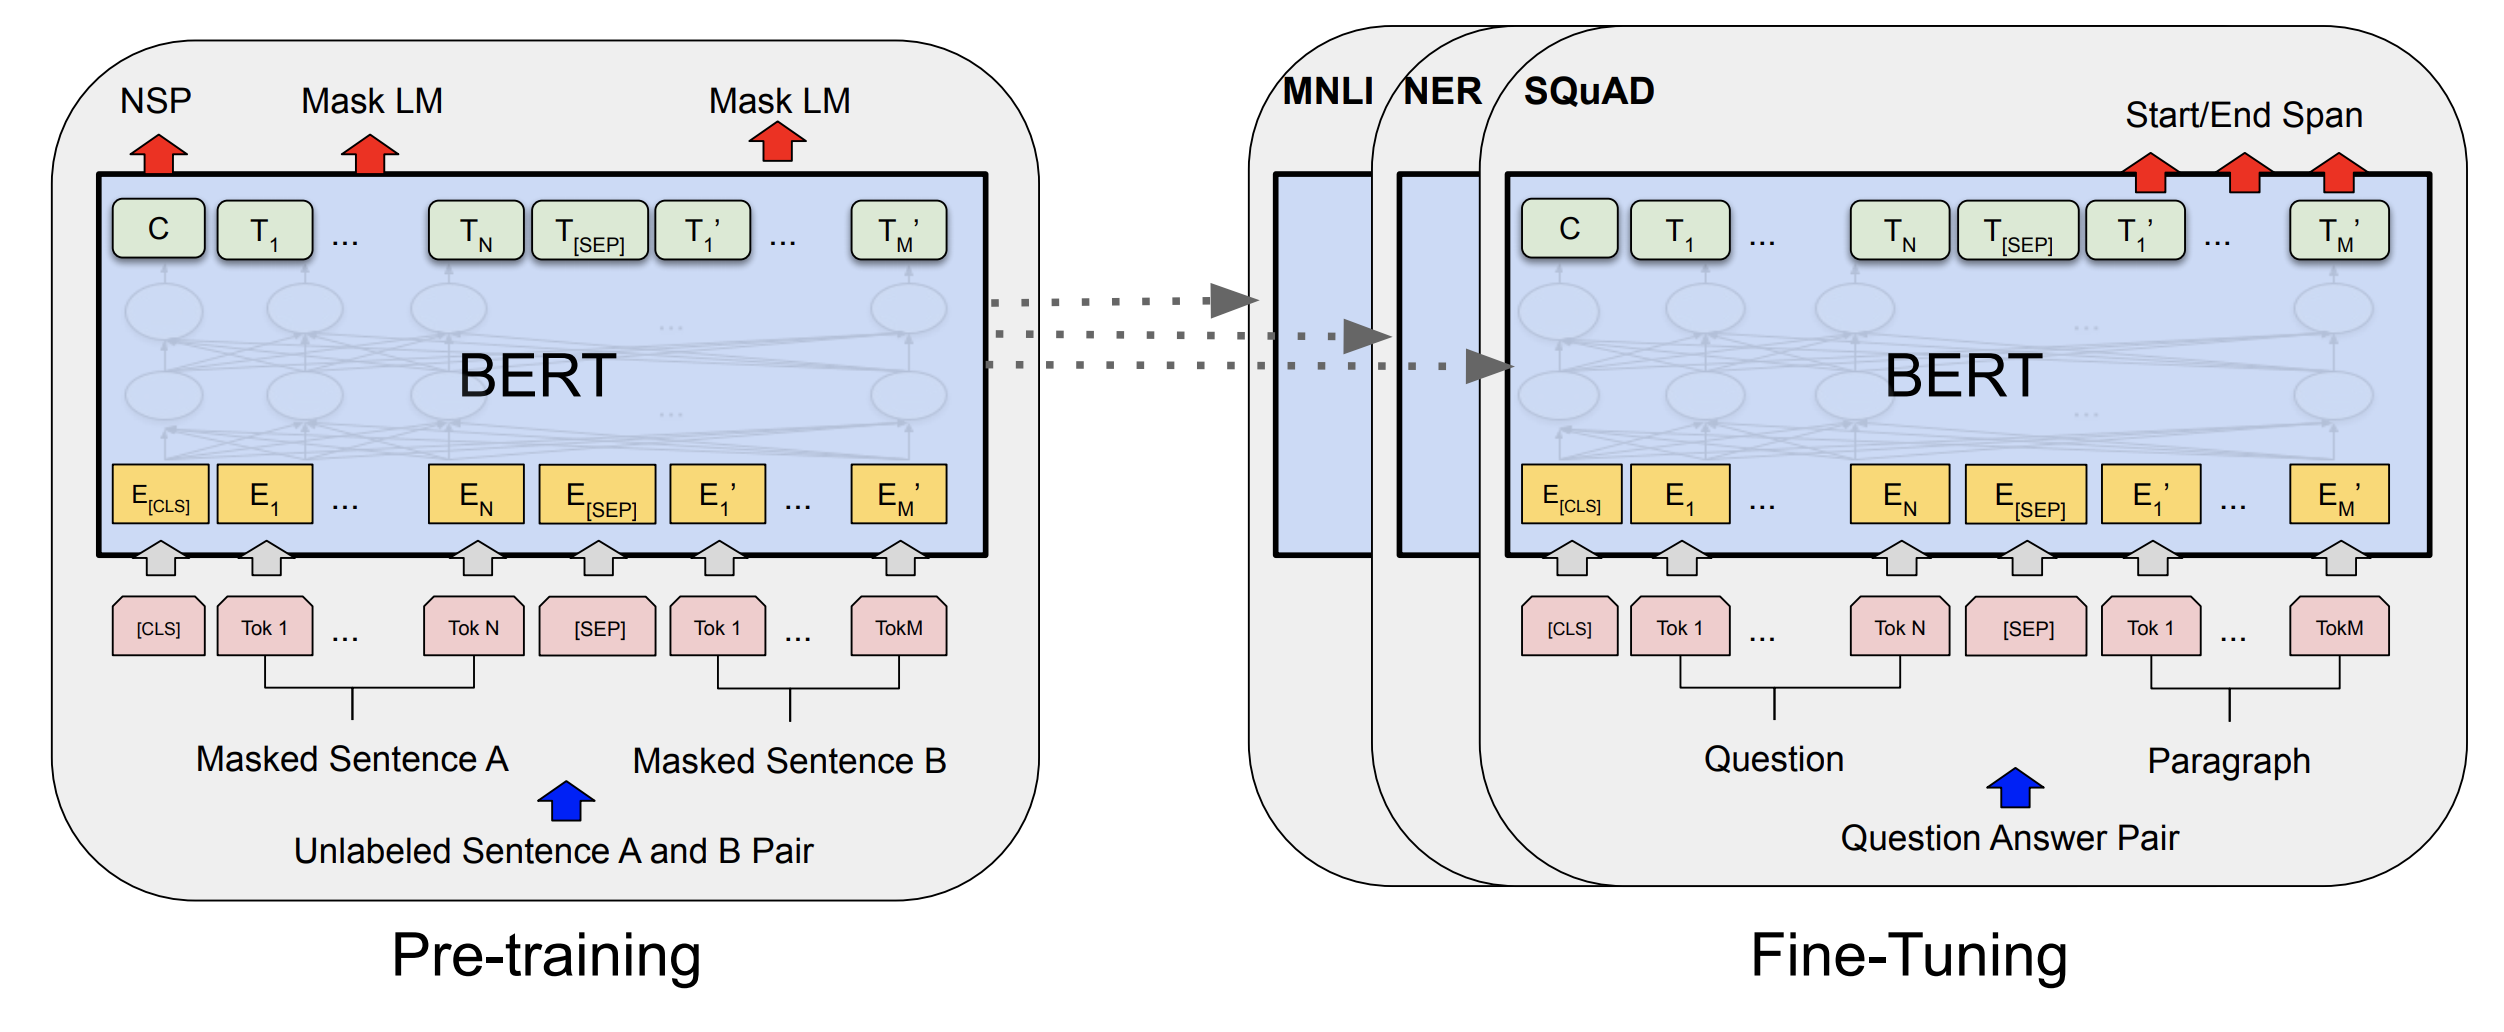
\includegraphics[scale=0.40]{bertprocedure.png}
  \caption{Overall pre-training and fine-tuning procedures for BERT. Apart from output layers, the same architectures are used in both pre-training and fine-tuning. The same pre-trained model parameters are used to initialize models for different down-stream tasks. During fine-tuning, all parameters are fine-tuned. \texttt{[CLS]} is a special symbol added in front of every input example, and \texttt{[SEP]} is a special separator token (e.g. separating questions/answers).}
  \label{fig:skip-gram}
\end{figure}
\subsubsection{Fine tuning \textbf{BERT}}
For each task, we simply plug its inputs and outputs into \textbf{BERT} and fine-tune all the parameter end-to-end. . At the output, the token representations are fed into an output layer for token level tasks, such as sequence tagging or question answering, and the \texttt{[CLS]} representation is fed into an output layer for classification, such as entailment or sentiment analysis.\\\\
Compared to pre-training, fine-tuning is relatively inexpensive. On my MacBook, it roughly only takes one and a half hour to run.
\section{Question Answering}
Building a question answering system is composed of two parts: \\\\
1. Finding documents that (potentially) contain an answer, which can be handled by traditional information retrieval \\
2. Finding an answer in a paragraph or a document, which is the focus of this section. \\
\textbf{The Stanford Attentive Reader} is quite successful, we will use the example below to demonstrate. \\\\
As figure 16 shows, we firstly find the word embedding of the question: \texttt{Which team won Super Bowl 50?}. We mark the start token using the first layer of \textbf{BERT}, and the end token of the question using the second layer of \textbf{BERT}. \\
 \begin{figure}
  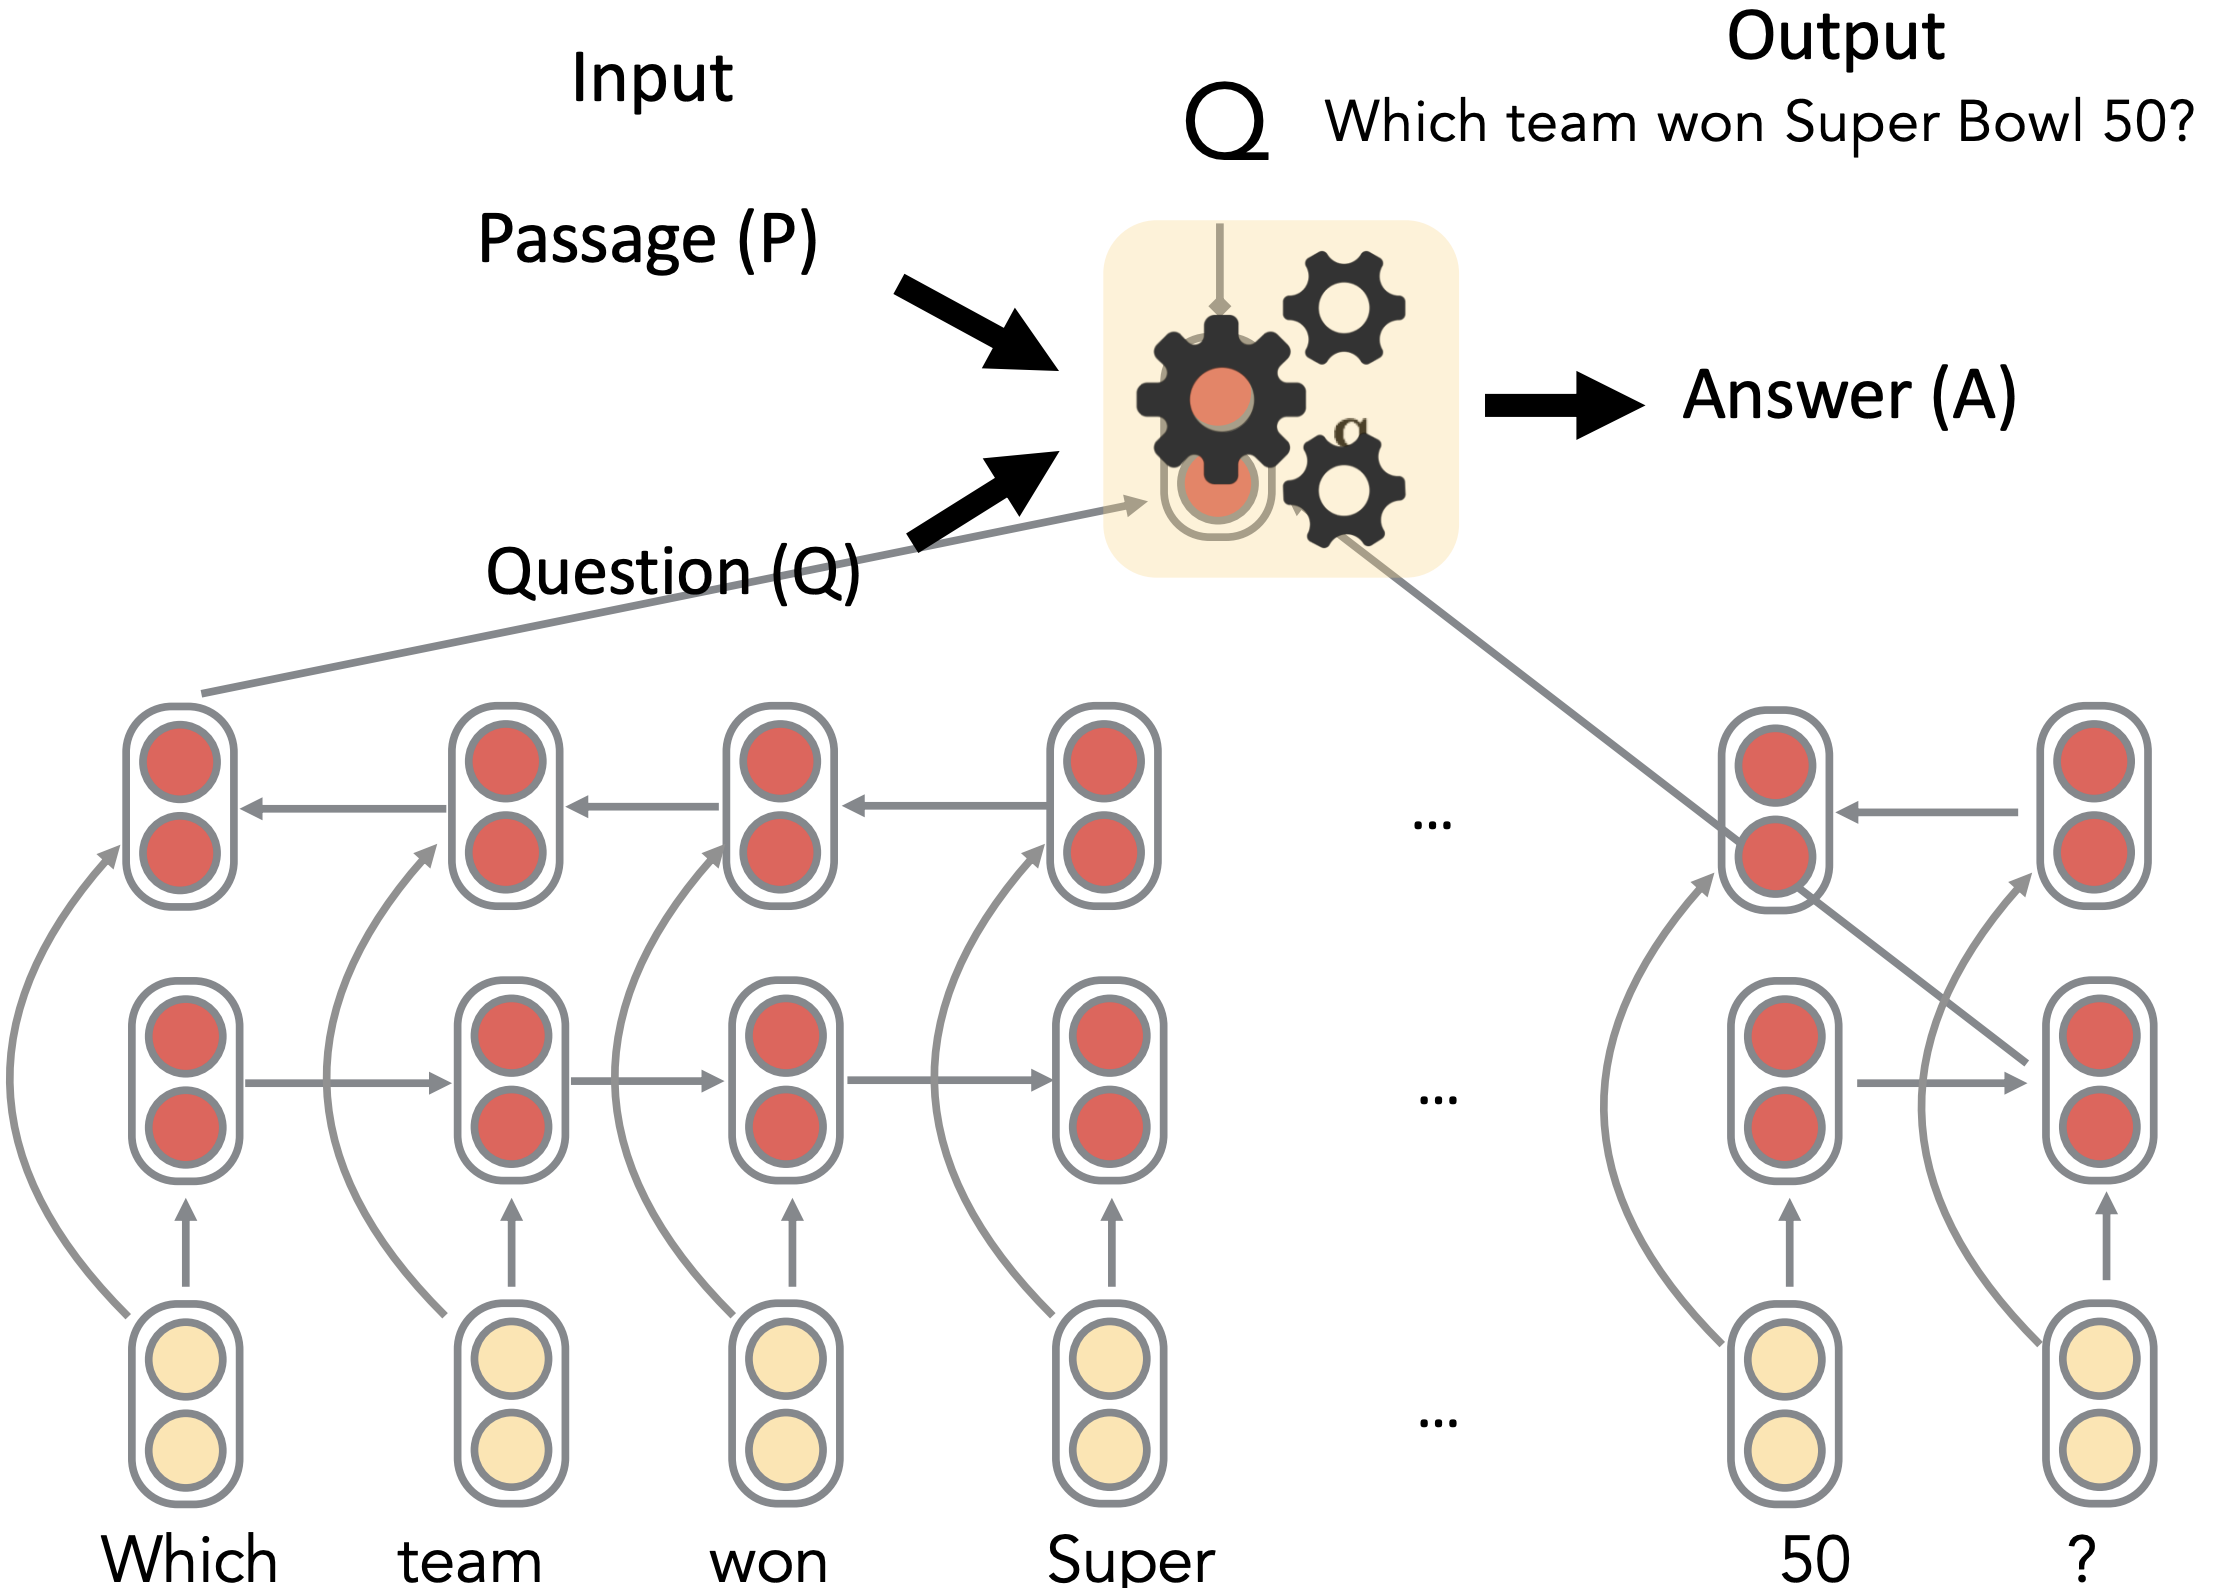
\includegraphics[scale=0.4]{q.png}
  \caption{A modelling of an example question: Which team won Super Bowl 50?}
  \label{fig:skip-gram}
\end{figure}
Then we aims to find the word embedding of the passage that contains the answer from the passage. \\
Then we calculate the attention score for each of the token in the paragraph, and define the start token of our output answer as 
\begin{align*}
a_i = softmax(\mathbf{q}^T \mathbf{W}_s \hat{p_i})
\end{align*}
the end token of our output answer as
\begin{align*}
a_i = softmax(\mathbf{q}^T \mathbf{W}_s' \hat{p_i})
\end{align*}
So why aren't we looking into the middle of the answer? When we are training, the stuff that are useful in the middle is already considered. And the vectors $W_s$ and $W_s'$ have taken account this. \\\\
 \begin{figure}
  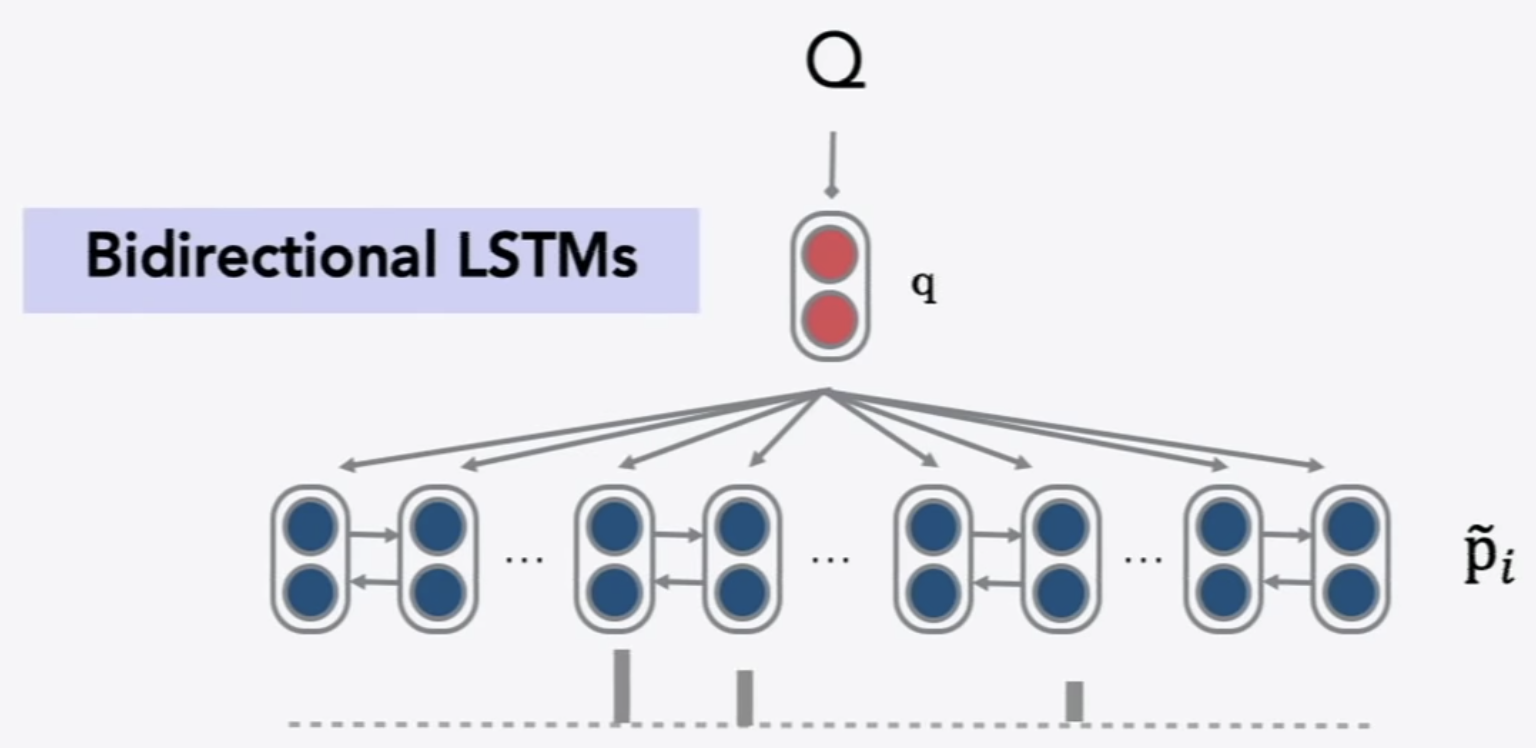
\includegraphics[scale=0.6]{a.png}
  \caption{A modelling of an example paragraph}
  \label{fig:skip-gram}
\end{figure}
The intuitive training goal is to maximize the probability of the predicted start and end token being the actual start and end token of the answer. This can be defined as the following formula:
\begin{align*}
\iota = - \sum log P^{(start)} (a_{start}) - \sum log P^{(end)} (a_{end})
\end{align*}

The attached jupiter notebook is an implementation of the above algorithm that runs on Kaggle's server: https://www.kaggle.com/c/tensorflow2-question-answering/overview.


\clearpage

\section{Reference}
Bengio, Yoshua, et al. "A neural probabilistic language model." Journal of machine learning research 3.Feb (2003): 1137-1155.\\\\
Mikolov, Tomas, et al. "Distributed representations of words and phrases and their compositionality." Advances in neural information processing systems. 2013.\\\\
Pennington, Jeffrey, Richard Socher, and Christopher Manning. "Glove: Global vectors for word representation." Proceedings of the 2014 conference on empirical methods in natural language processing (EMNLP). 2014. \\\\
Peters, Matthew E., et al. "Deep contextualized word representations." arXiv preprint arXiv:1802.05365 (2018).\\\\
Devlin, Jacob, et al. "Bert: Pre-training of deep bidirectional transformers for language understanding." arXiv preprint arXiv:1810.04805 (2018).\\\\
Vaswani, Ashish, et al. "Attention is all you need." Advances in neural information processing systems. 2017.




\end{document} 